\chapter{Benchmarking of Simplified-Model Controllers for Locomotion\label{chapter:simplified_benchmarking}}

In Part~\ref{part:wbc}, we discussed whole-body controllers that take into account different types of robots, as well as the interaction between the robot and the environment. Independently of the choice of the whole-body controller, we assumed a high-level algorithm that provides the reference for the Cartesian trajectories, e.g., CoM and foot trajectories. This part presents the design of two high-level controllers that compute the commands for the whole-body control layer presented in Part~\ref{part:wbc}. This chapter, in particular, defines the three-layer controller architecture illustrated in Figure~\ref{fig:three-layer} as shown in Figure~\ref{fig:three-layer-simplified-benchmarking}.
The \emph{whole-body QP control} ensures the tracking of the desired CoM and foot trajectories by considering the complete robot models. A detailed design of different kinds of whole-body controllers is discussed in Part~\ref{part:wbc}.
The \emph{trajectory optimization} layer is maintained fixed with a unicycle-based planner~\citep{8594277} that generates the desired DCM and foot trajectories. 
The \emph{simplified model controller} is responsible for implementing a control law that stabilizes the unstable DCM dynamics. We approach the stabilization problem by designing two different controllers: an \emph{instantaneous} and a \emph{predictive} one.
We compare several combinations of the control architecture with the kinematics-based whole-body QP control layer presented in Section~\ref{sec:ik_qp}.
We carried out the test on the humanoid robot iCub v2.7 -- see Section~\ref{sec:icub2.7}.
\par
The chapter is organized as follows. Section~\ref{sec:background-bachmarking} introduces a state-of-the-art implementation of the footstep planner and the DCM planner implemented in the~\emph{trajectory optimization layer}. Section~\ref{sec:simplified_model_architecture} details the components constituting the simplified model blocks of the three-layer controller architecture. Section~\ref{sec:results_simplified_benchmarking} presents the experimental validation of the proposed approaches and shows an explanatory table comparing the different simplified control strategies. Finally, Section~\ref{sec:conclusion_simplified_benchmarking} concludes the chapter.
\par
The content of this chapter appears partially in:
\begin{leftbar}
	\begin{quote}%
		\bibentry{8625025} \vspace{5mm}\newline 
		\bibentry{Romualdi2020ARobots} \vspace{5mm} \newline
		\begin{tabular}{c p{10.0cm}}
			     Video & \href{https://www.youtube.com/watch?v=FIqwAO71Fc4}{\texttt{https://www.youtube.com/watch?v=FIqwAO71Fc4}} \\
			     GitHub &  \href{https://github.com/robotology/walking-controllers}{\texttt{robotology/walking-controllers}} 
		\end{tabular}
	\end{quote}
\end{leftbar}

\begin{figure}[t]
    \centering
    \includegraphics{chapter_simplified_benchmarking/figures/three-layer.tikz}
    \caption[The three layer controller architecture for bipedal locomotion in rigid environment]{The control architecture is composed of three layers: the \emph{trajectory optimization}, the \emph{simplified model control}, and the \emph{whole-body control}. The inner layer is described in Chapter~\ref{chapter:benchmarking_wbc}.
    \label{fig:three-layer-simplified-benchmarking}}
\end{figure}


\section{System modeling\label{sec:flex_joint_system_modeling}}

TALOS's hip flexibility has a significant impact on its leg control and, as a result, its balance and locomotion~\citep{Ramuzat2021ComparisonTALOS}. In this section, we model the TALOS's hip flexibility by means of underactuated joints. The section also extends the humanoid robot model dynamics presented in Section~\ref{sec:multi-body-dynamics} to consider the robot's link visco-elasticity.

\subsection{Model of the hip flexibility}

Following the work of~\cite{Villa2022TorqueFlexibility}, we model the flexibility by introducing two passive virtual joints between the base link and each leg. The virtual joints simulate the motion caused by the visco-elastic deformation of the waist-leg connection, where the link cross section is reduced.
Given the $i$-th passive joint, we assume that it exerts a torque $\tau^f_i$ that depends on the
joint deflection $s^f_i$ and its velocity $\dot{s}^f_i$~\citep{Nakaoka2007Constraint-basedMechanisms} as
\begin{equation}
\label{eq:flexible_joint}
\tau^f_i = -k_i s^f_i - d_i \dot{s}^f_i.
\end{equation}
where $k_i$ and $d_i$ are, respectively, the stiffness and damping coefficients of the flexible
joint $i$. By assuming to model the link flexibility with $n_f$ joints, we can consider the robot to
have $n$ joints where $n = n_a + n_f$ with $n_a$ are the actuated joints.
\par
In the specific case of the TALOS robot, the authors of \citep{Villa2022TorqueFlexibility} notice that
the stiffness is due to the vertical linkage and, consequently, they model the flexibility along
the pitch and roll axis, only. In this chapter, the same consideration holds, so we introduce two
passive flexible joints for each leg. As a result $n_f = 4$ while $n_a = 32$ -- see Section~\ref{sec:talos}.
\par
Assuming that it is possible to estimate $\tau^f_i$, we approximate the flexible joint state by discretizing
Equation~\eqref{eq:flexible_joint}, resulting in
\begin{IEEEeqnarray}{C}
\phantomsection \label{eq:flexibility_discretized} \IEEEyesnumber \IEEEyessubnumber*
s^f_i[k] = \frac{d_i s^f_i[k-1] - \tau^f_i[k] \diff t}{k_i \diff t + d_i}, \label{eq:flexibility_discretized_position} \\
\dot{s}^f_i[k] = \frac{s^f_i[k] - s^f_i[k-1]}{\diff t}.
\end{IEEEeqnarray}
Here $\diff t$ is the sampling time. $s^f_i[k] = s^f_i(t_0 + k \diff t)$ and $\dot{s}^f_i[k] = \dot{s}^f_i(t_0 + k \diff t)$.


\subsection{Modeling of a floating base system with flexible joints}
This section extends the floating base system model presented in Section~\ref{sec:multi-body-dynamics} to consider underactuated flexible joints.
\par
Let us consider an inertial frame $\mathcal{I}$ and a floating base system making $n_c$ contact with the environment. We recall:
\begin{itemize}
    \item $B = (p_B, [B])$ is the frame rigidly attached to the robot base. ${}^\mathcal{I} H _B \in \SE(3)$  describes the position and orientation of $B$ with respect to the inertial frame $\mathcal{I}$.
    \item Hereafter the base velocity expressed in mixed representation ${}^{B[\mathcal{I}]}\mathrm{v}_{\mathcal{I}, B}$ such that  ${}^{B[\mathcal{I}]}\mathrm{v}_{\mathcal{I}, B}^\top = \begin{bmatrix}
    {}^{\mathcal{I}} \dot{p}_B^\top & {}^{B[\mathcal{I}]}\dot{\omega}_{\mathcal{I}, B}^\top.
    \end{bmatrix}$
    \item The actuated and flexible joint positions are indicated, respectively, with $s^a \in \mathbb{R}^{n_a}$ and $s^f \in \mathbb{R}^{n_f}$;
    \item the actuated and flexible joint torques are indicated, respectively, with $\tau^a \in \mathbb{R}^{n_a}$ and $\tau^f \in \mathbb{R}^{n_f}$.
\end{itemize}
We extend the robot configuration~\eqref{eq:robot_configuration_mixed} by introducing the flexible
joint value as $q = ({}^{\mathcal{I}} p_B, {}^{\mathcal{I}} R_{B}, s^a, s^f)$. $q$ is an element
of a Lie group $\lieGroup{Q} = \mathbb{R}^3 \times SO{(3)} \times \mathbb{R}^{n_a} \times
\mathbb{R}^{n_f}$. The associated lie Algebra writes as $\lieAlgebra{q} = \mathbb{R}^3 \times \so(3)
\times \mathbb{R}^{n_a} \times \mathbb{R}^{n_f}$. Here, we recall that $\lieAlgebra{q}$ is isomorphic to $\mathbb{R}^3 \times \mathbb{R}^3 \times \mathbb{R}^{n_a} \times \mathbb{R}^{n_f}$ -- see Appendix~\ref{sec:tangent_space_lie}.
\par
The \emph{velocity of the multi-body system} belongs to $\lieAlgebra{q}$ and we denote it with $\nu = \left({}^{\mathcal{I}} \dot{p}_B, {}^{B[\mathcal{I}]}{\omega}_{\mathcal{I}, B}, \dot{s}^a, \dot{s}^f\right)$.
\par
Slightly modifying~\eqref{eq:system}, we write the dynamics of a floating base system with flexible joints as follows 
\begin{equation}
\label{eq:system_flex}
{M}({q})\dot{{\nu}} + h({q}, {\nu}) =  \begin{bmatrix}
{0}_{6\times n_a} \\ I_{n_a} \\ 0_{n_f\times n_a}
\end{bmatrix}{\tau}^a + 
\begin{bmatrix}
{0}_{6\times n_f} \\ 0_{n_a\times n_f} \\ I_{n_f} 
\end{bmatrix}{\tau}^f +
             {J}_{\mathcal{C}}(q)^\top \mathrm{f},
\end{equation}
where
\begin{equation}
	{J}_{\mathcal{C}}({q}) = 
	\begin{bmatrix}{J}_{\mathcal{C}_1}({q}) \\ \vdots \\ {J}_{\mathcal{C}_{n_c}}({q})  \end{bmatrix}, \quad
	\mathrm{f} = \begin{bmatrix}
		{}_{\mathcal{C}_1[\mathcal{I}]}\mathrm{f}_1 \\
		\vdots\\
		{}_{\mathcal{C}_{n_c}[\mathcal{I}]}\mathrm{f}_{n_c}
	\end{bmatrix}.
\end{equation}
Recalling that $n=n_a + n_f$, $M\in \mathbb{R}^{(n+6) \times (n+6)}$ is the mass matrix,
$h \in \mathbb{R}^{(n+6)}$ accounts for Coriolis, the centrifugal effects and the gravity term.  ${}_{\mathcal{C}_k[\mathcal{I}]}\mathrm{f}_k \in \mathbb{R}^{6}$ denotes the $k$-th external wrench applied by the environment on the robot expressed in mixed representation.
The Jacobian $J_{\mathcal{C}_k}$ is the mixed velocity Jacobian of the contact $\mathcal{C}_k$.
\par
Following the same approach presented in Section~\ref{sec:multi-body-dynamics}, the
dynamics~\eqref{eq:system_flex} is expressed by separating the first $6$ rows, which refers to the underactuated floating base, from the last rows $n_a + n_f$, which refers to the actuated and flexible joints as:
\begin{IEEEeqnarray}{c}
\IEEEyesnumber \phantomsection
M_{\nu}(q) \dot{\nu} + h_{\nu} (q, \nu) =  J^\top_{{\mathcal{C}}_\nu}(q) \;  \mathrm{f},\label{eq:system_flex_base_projection} \IEEEyessubnumber \\
M_{s}(q) \dot{\nu} + h_{s} (q, \nu) = \begin{bmatrix}
I_{n_a} \\ 0_{n_f\times n_a}
\end{bmatrix}{\tau}^a +
\begin{bmatrix}
 0_{n_a\times n_f} \\ I_{n_f}
\end{bmatrix}{\tau}^f +  J^\top_{{\mathcal{C}}_s}(q)  \; \mathrm{f}. \label{eq:system_flex_joint_projection} \IEEEyessubnumber
\end{IEEEeqnarray}
The subscript $\nu$ refers to the first $6$ rows of the matrix, while $s$ refers to the last $n$
rows. Equation~\eqref{eq:system_flex_base_projection} is often denoted as the base projection of the floating base dynamics, while
Equation~\eqref{eq:system_flex_joint_projection} is the joint space projection.

\section{Simplified model architecture \label{sec:simplified_model_architecture}}
In this section, we summarize the components constituting the simplified model blocks of the three-layer controller architecture -- Figure~\ref{fig:three-layer}. In detail, we present
\begin{itemize}
    \item how we consider the first and last steps in the DCM planner,
    \item the swing foot trajectory planner,
    \item the simplified model control layer.
\end{itemize}
These components share a lot of commonalities with other state-of-the-art
approaches. Nevertheless, this section presents how these three components
interconnect to define part of a walking architecture.


\subsection{The DCM trajectory planner\label{sec:dcm_traj_planner_simplfied}}
The DCM trajectory planner used in our architecture inherits from the formulation presented in Section~\ref{sec:dcm_traj_gen}. However, differently from~\cite{Englsberger2014}, we explicitly consider specific boundary conditions for the first and last steps.
\par
For the first double support phase, we ask for an initial DCM position ${\xi}^{\text{ios}_\text{DS}}_1$ that coincides with the projection of the measured CoM on the ground surface. In this particular context, we set the initial boundary conditions of the DCM position~\eqref{eq:3d_dcm_ds_boundary_ios} and velocity~\eqref{eq:3d_dcm_ds_boundary_ios_v} as:
\begin{IEEEeqnarray}{LL}
\phantomsection  \IEEEyesnumber  \IEEEyessubnumber*
  {\xi}^{\text{ios}_\text{DS}}_1 = x_\text{LIP} \\
  \dot{{\xi}}^{\text{ios}_\text{DS}}_1 = {0}_{2\times1}.
\end{IEEEeqnarray}
Figure~\ref{fig:dcm_first_step} presents the DCM trajectory generation for the first double support phase. 
\begin{figure}[t]
\centering
    \begin{subfigure}[b]{0.48\textwidth}
        \centering
        \includegraphics{chapter_simplified_benchmarking/figures/dcm_first_step.tikz}
        \caption{DCM trajectory at the first step}
        \label{fig:dcm_first_step}
    \end{subfigure}
    \hfill
    \begin{subfigure}[b]{0.48\textwidth}
        \centering
        \includegraphics{chapter_simplified_benchmarking/figures/dcm_last_step.tikz}
        \caption{DCM trajectory at the last step}
        \label{fig:dcm_last_step}
    \end{subfigure}
	\caption[DCM trajectory planner at the first and last step]{DCM trajectory planner at the first and last step. The SS trajectory is represented by the orange segments, while the DS trajectory is represented by the light blue curves (a) At the first step, the initial DCM position ${\xi}^{\text{ios}_\text{DS}}_1$ coincides with the projection of the CoM on the ground surface. (b) At the last step, the final DCM position ${\xi}^{\text{eos}_{\text{DS}}}_N$ coincides with the projection of the CoM on the ground surface.}
	\label{fig:dcm_first_last_step}
\end{figure} 
\par
Similarly, the desired position of the DCM at the end of the double support phase
${\xi}^{\text{eos}_{\text{DS}}}_N$ must coincide with the projection of the desired CoM on the ground surface, denoted by $x_\text{LIP}^*$. This is obtained as the middle point between the two feet.
In this particular case, we set the final boundary conditions for the DCM position~\eqref{eq:3d_dcm_ds_boundary_eos} and velocity~\eqref{eq:3d_dcm_ds_boundary_eos_v} as:
\begin{IEEEeqnarray}{LL}
\phantomsection  \IEEEyesnumber  \IEEEyessubnumber*
  {\xi}^{\text{eos}_\text{DS}}_N = x_\text{LIP}^* \\
  \dot{{\xi}}^{\text{eos}_\text{DS}}_N = {0}_{2\times1}.
\end{IEEEeqnarray}
In \cite{Englsberger2014}, the DCM trajectory for the last single support phase is calculated by assuming that the final position of the DCM coincides with the local ZMP in the last step -- Equation~\eqref{eq:dcm_eos_evaluation_final_condition}. In our test, we noticed that this choice may lead to an undesired overshoot of the DCM projection into the \emph{coronal plane}~\footnote{A \emph{coronal plane}, also known as the \emph{frontal plane}, is any vertical plane that divides the body into ventral and dorsal sections.}, and consequently to an unfeasible DCM trajectory. 
To mitigate this behavior, we ask that the final condition of the single support DCM trajectory ${\xi}_{N-1}^{\text{eos}}$ belongs to the \emph{affine combination} (see Section~\ref{sec:affine_convex_sets}) of the two last footprints, i.e., 
\begin{equation}
    {\xi}_{N-1}^{\text{eos}} = \alpha_\text{LS} x_{\text{ZMP}_N}  + (1 - \alpha_\text{LS}) x_{\text{ZMP}_{N-1}}.
\end{equation}
When $\alpha_\text{LS} = 0$ the DCM position coincides with the ZMP position of the stance foot. On the other hand, if $\alpha_\text{LS} = 1$ we obtain the same condition proposed by \cite{Englsberger2014}. In Figure~\ref{fig:dcm_final_step_alpha}, we present the DCM trajectory in the last step projected on \emph{frontal plane} for different values of $\alpha_\text{LS}$.  $\alpha_\text{LS} = 1$ leads to an undesired overshoot and, as a consequence, to an unfeasible DCM trajectory. In our experiments, we always set $\alpha_\text{LS} = 0.2$, which in our opinion is a good compromise between a responsive trajectory while avoiding undesired overshoots. 
\begin{figure}[t]
  \centering
    \includegraphics{chapter_simplified_benchmarking/figures/dcm_final_step_alpha.tikz}
    \caption[Final step DCM trajectory w.r.t. $\alpha_\text{LS}$]{Final step DCM trajectory w.r.t. $\alpha_\text{LS}$. The greater $\alpha_\text{LS}$, the higher the overshoot. \label{fig:dcm_final_step_alpha}}
\end{figure}
Figure~\ref{fig:dcm_last_step} presents the generation of the DCM trajectory for the last double support phase. 

\subsection{Swing Foot Trajectory \label{sec:swing_foot_trajectory}}
We now discuss the problem of generating the foot trajectory from the footsteps. More formally, given two consecutive footsteps poses, hereafter denoted with ${}^\mathcal{I} H _{F_0} \in \SE(3)$ and ${}^\mathcal{I} H _{F_1} \in \SE(3)$, we aim to find a trajectory that connects these two poses. A common approach to this problem is to seek a foot trajectory ${}^\mathcal{I} H _{F}(t)$ such that its acceleration or jerk\footnote{We denote with \emph{jerk} the rate at which an object's acceleration changes with respect to time} is minimized. Since all the whole-body control layer implementations presented in Part~\ref{part:wbc} assume that frame velocity is expressed in \emph{mixed representation} -- Section~\ref{sec:mixed_spatial_velocity}, we split the problem of finding an optimal Cartesian trajectory into two subproblems, namely: evaluating a positional trajectory $p_F(t) \in \mathbb{R}^3$ and a rotation trajectory ${}^\mathcal{I} R _ F (t) \in \SO(3)$.

\subsubsection{Swing foot position}
During the walking gait, the swing foot has to move from the initial position $p_F(t_0) = p_{F_0}$ to $p_F(t_N) = p_{F_N}$ to reach a desired maximum
height. The instant in which a foot reaches its maximum altitude is called the apex time, $t_\text{apex}$.
\par
We want to find a trajectory $p_F(t) \in \mathbb{R}^3$ such that:
\begin{itemize}
    \item $p_F(t_0) = p_{F_0}$, $p_F(t_N) = p_{F_N}$ and $p_F(t_\text{apex}) = p_{F_\text{apex}}$
    \item the integral of a suitable Lagrangian function $\mathcal{L}(t)$ is minimized, i.e., 
    \begin{equation}
        \label{eq:foot_position_minimization_general}
        \minimize \int_{T_{0}}^{T_{N}} \mathcal{L}(t) \diff t,
    \end{equation}
    where $\mathcal{L}(t) \ge 0$.
\end{itemize}
Depending on the choice of the objective function, we can design a minimum acceleration or a minimum jerk trajectory.
\paragraph{Minimum acceleration trajectory}
If we set the Lagrangian function $\mathcal{L}(t)$ as the squared-norm of the linear acceleration:
\begin{equation}
    \mathcal{L} = \ddot{p}_F^\top \ddot{p}_F,
\end{equation}
it is possible to show that a trajectory composed by the concatenation of the $3^\text{rd}$ order polynomial functions
\begin{equation}
    \label{eq:spline_3d_order}
    s_i: p_F (t) =  a _{i, 3} t ^ 3 + a _ {i,2} t ^ 2 + a _ {i,1} t + a _ {i,0},
\end{equation}
is a minimum acceleration trajectory. Here the coefficients $a_{i,j}$ are chosen to satisfy the position and velocities boundary conditions for each subtrajectory,
The complete foot position minimum acceleration trajectory is finally computed by attaching the 3rd-order polynomial functions~\eqref{eq:spline_3d_order} as 
\begin{equation}
    p_F (t) = \begin{cases}
      a _{0, 3} t ^ 3 + a _ {0,2} t ^ 2 + a _ {0,1} t + a _ {0,0} \quad  \text{if } t_0 \le t \le t_\text{apex} \\
      a _{1, 3} t ^ 3 + a _ {1,2} t ^ 2 + a _ {1,1} t + a _ {1,0} \quad  \text{if }  t_\text{apex} < t \le t_N
    \end{cases}
\end{equation}
\par
Appendix~\ref{appendix:min_acc} presents all the passages required to evaluate a minimum acceleration trajectory in $\mathbb{R}^n$.
\paragraph{Minimum jerk trajectory}
If we set the Lagrangian function $\mathcal{L}(t)$ as the squared-norm of the linear jerk:
\begin{equation}
    \mathcal{L} = \dddot{p}_F^\top \dddot{p}_F
\end{equation}
we notice that a trajectory composed by the concatenation of a $5^\text{th}$ order polynomial functions:
\begin{equation}
\label{eq:spline_5d_order}
    s_i :  p_F (t) =  a _ {i,5} t ^ 5 + a _ {i,4} t ^ 4 + a _ {i,3} t ^ 3 + a _ {i,2} t ^ 2 + a _ {i,1} t + a _ {i,0},
\end{equation}
minimizes the jerk. The coefficients $a_{i,j}$ are chosen to satisfy the boundary conditions of position, velocity and acceleration.
Finally, the complete foot position minimum acceleration trajectory is computed by attaching $5^\text{th}$-order polynomial functions as:
\begin{equation}
    p_F (t) = \begin{cases} 
      a _ {0,5} t ^ 5 + a _ {0,4} t ^ 4  + a _{0, 3} t ^ 3 + a _ {0,2} t ^ 2 + a _ {0,1} t + a _ {0,0} \quad  \text{if } t_0 \le t \le t_\text{apex} \\
      a _ {1,5} t ^ 5 + a _ {1,4} t ^ 4  + a _{1, 3} t ^ 3 + a _ {1,2} t ^ 2 + a _ {1,1} t + a _ {1,0} \quad  \text{if }  t_\text{apex} < t \le t_N
    \end{cases}
\end{equation}
Appendix~\ref{appendix:min_jerk} presents all the passages required to evaluate a minimum jerk trajectory in $\mathbb{R}^n$.
\subsubsection{Swing foot orientation}
During the walking gait, the swing foot rotates from the initial orientation ${}^\mathcal{I}R_F(t_0) = {}^\mathcal{I}R_{F_0}$ to ${}^\mathcal{I}R_F(t_N) = {}^\mathcal{I}R_{F_N}$. Similarly to what we discussed for the generation of position trajectory, we now aim to compute a trajectory ${}^\mathcal{I}R_F(t)$ such that 
\begin{itemize}
    \item  ${}^\mathcal{I}R_F(t_0) = {}^\mathcal{I}R_{F_0}$ and ${}^\mathcal{I}R_F(t_N) = {}^\mathcal{I}R_{F_N}$
    \item a suitable Lagrangian function $\mathcal{L}(t)$ is minimized.
\end{itemize}
We can now construct a minimum acceleration or a minimum jerk trajectory depending on the objective function, $\mathcal{L}(t)$.
\paragraph{Minimum acceleration trajectory}
If we set the Lagrangian function $\mathcal{L}(t)$ as the squared-norm of the right trivialized (inertial frame) angular acceleration ${}^\mathcal{I} \dot{\omega}_{\mathcal{I}, F}$:
\begin{equation}
    \label{eq:lagrangian_min_acc}
    \mathcal{L} = {}^\mathcal{I} \dot{\omega}_{\mathcal{I}, F}^\top {}^\mathcal{I} \dot{\omega}_{\mathcal{I}, F}
\end{equation}
and we ask for a zero initial and final angular velocity, 
it is possible to show that the  
\begin{equation}
    \label{eq:min_acc_rot}
    {}^\mathcal{I}R_F(t) = \exp{\left(s(t-t_0) \log\left( {}^\mathcal{I}R_F(t_N) {}^\mathcal{I}R_{F_0}^\top  \right)\right)} {}^\mathcal{I}R_{F_0},
\end{equation}
where $s(\tau)$ is given by
\begin{equation}
\label{eq:min_acc_rot_s}
    s(\tau) = \frac{3}{(t_N - t_0)^2} \tau^2 - \frac{3}{(t_N - t_0)^3} \tau^3,
\end{equation}
minimizes the integral of the Lagrangian function~\eqref{eq:lagrangian_min_acc}~\citep[Section~9.2]{Lynch2017ModernControl}\citep{Zefran1999MetricsKinematics,Zefran1998OnMotions,Park1997SmoothRotations}
\par
In Appendix~\ref{appendix:optimal_planning_so3}, we present the theory behind the minimum acceleration trajectory in $\SO(3)$. 
\paragraph{Minimum jerk trajectory}
If we set the Lagrangian function $\mathcal{L}(t)$ as the squared norm of the right trivialized (inertial frame) angular jerk ${}^\mathcal{I} \ddot{\omega}_{\mathcal{I}, F}$:
\begin{equation}
    \label{eq:lagrangian_min_jerk}
    \mathcal{L} = {}^\mathcal{I} \ddot{\omega}_{\mathcal{I}, F}^\top {}^\mathcal{I} \ddot{\omega}_{\mathcal{I}, F}.
\end{equation}
and we ask for a zero initial and final angular velocity and acceleration, 
it is possible to show that  
\begin{equation}
    \label{eq:min_jerk_rot}
    {}^\mathcal{I}R_F(t) = \exp{\left(s(t-t_0) \log\left( {}^\mathcal{I}R_F(t_N) {}^\mathcal{I}R_{F_0}^\top  \right)\right)} {}^\mathcal{I}R_{F_0}
\end{equation}
where $s(\tau)$ is given by
\begin{equation}
\label{eq:min_jerk_rot_s}
    s(\tau) = \frac{6}{(t_N - t_0)^5} \tau^5 - \frac{15}{(t_N - t_0)^4} \tau^4 + \frac{10}{(t_N - t_0)^3} \tau^3,
\end{equation}
minimizes the integral of the Lagrangian function~\eqref{eq:lagrangian_min_jerk}~\citep{Liu2017Minimum-jerkActuator,Zefran1999MetricsKinematics}
\par
Differently from~\eqref{eq:min_acc_rot} and~\eqref{eq:min_acc_rot_s}, to prove~\eqref{eq:min_jerk_rot} and~\eqref{eq:min_jerk_rot_s} we need to exploit the mathematical tools of \emph{Differential Geometry}. Since this topic is outside the scope of the thesis, we avoid presenting the rigorous proof. The interested reader can refer to the extensive literature, among which it is worth mentioning~\citep{Zefran1999MetricsKinematics,Zefran1998OnMotions,Pressley2010ElementaryGeometry,Needham2021VisualForms,Selig2007CurvesSE3,Dubrovin1984ModernApplications}





\subsection{Simplified model control layer}

As introduced in Section~\ref{sec:dcm}, the simplified model~\eqref{eq:dcm_dynamics_lipm_com} shows that the CoM asymptotically converges to a constant DCM, while the DCM has an unstable first-order dynamics~\eqref{eq:dcm_dynamics_lipm_dcm}. In this section, we present control laws that aim at stabilizing the DCM dynamics by assuming the location of the ZMP $x_\text{ZMP}$ as the control input.
\par
This stabilization problem has been tackled by designing and comparing \emph{instantaneous} and \emph{predictive} (MPC) control laws.
Unlike the MPC, the instantaneous control law does not solve any optimization problem, and it uses only the current desired and actual position of the DCM to evaluate its output.
\par

\subsubsection{DCM instantaneous control}
\label{instantaneous-control}

Differently from \cite{Englsberger2015}, we propose an instantaneous control law that does not perform a cancellation of the unstable system dynamics, which, in practice, is never perfect and can lead to system instabilities. More precisely, we chose
\begin{equation}
\label{eq:reactive_dcm}
x_\text{ZMP}^{*} = \xi^{\text{ref}}- \frac{1}{\zeta} \dot{\xi}^{\text{ref}}+ K^{\xi}_{p} \left(\xi - \xi^\text{ref} \right) + K^{\xi}_{i} \int{\xi - \xi^\text{ref} \diff t}.
\end{equation}
where $K^{\xi}_{p}> I_2$ and $K^{\xi}_{i} > 0_{2\times2}$
\par
Applying the control input \eqref{eq:reactive_dcm} to the system \eqref{eq:dcm_dynamics_lipm_dcm_without_lip} leads to the following closed-loop dynamics:
\begin{equation}
\label{eq:reactive_cl}
\dot{\xi} - \dot{\xi}^{\text{ref}} = \zeta(I_2 - K^{\xi}_{p})  (\xi - \xi^{\text{ref}})
-\zeta K^{\xi}_{i}  \int{\xi - \xi^{\text{ref}} \diff t}.
\end{equation}
It is easy to show that the DCM error and its integral converge asymptotically to zero.
The above law~\eqref{eq:reactive_dcm} is very simple to implement and guarantees the tracking of the
desired DCM. 
The main limitation is that it may not ensure the feasibility of the gait, since the position of the ZMP may exit the support polygon and, consequently, the ZMP contact feasibility criterion~\citep{Vukobratovic1969} may not be guaranteed.
Furthermore, the above instantaneous control law does not take into account the desired DCM trajectory planned for the future.

\subsubsection{DCM predictive control}
\label{predictive-control}
In order to overcome these issues, we design a model predictive controller by following the work of ~\cite{Krause2012}. 
The control objective is achieved by framing the controller as a constrained optimization problem composed of three
main elements, namely: \emph{the prediction model}, an \emph{objective
function} and a set of \emph{inequality constraints}.

\paragraph{Prediction model} In the MPC framework, we consider the dynamics of DCM \eqref{eq:dcm_dynamics_lipm_dcm_without_lip} as a prediction model. Equation~\eqref{eq:dcm_dynamics_lipm_dcm_without_lip} is discretized supposing piecewise constant ZMP trajectories. By applying the \emph{Zero order hold} technique presented in Section~\ref{sec:zoh}, the discrete DCM dynamics writes as follows:
\begin{equation}
\label{eq:dcm_discrete}
\begin{split}
\xi_{k+1} &= F \xi_k + G x_{\text{ZMP}_{k}} \\
&=
\begin{bmatrix}
e^{\zeta T} & 0 \\
0 & e^{\zeta T}
\end{bmatrix} \xi_k {+}
\begin{bmatrix}
1 - e^{\zeta T} & 0\\
0 & 1 - e^{\zeta T}
\end{bmatrix}
x_{\text{ZMP}_{k}}.
\end{split}
\end{equation}
where $T$ is the fixed sampling time. 
\paragraph{Objective function}
The objective function is defined in terms of two main tasks, namely a tracking task and a control input regularization task. 
\par
To follow a desired DCM trajectory, we minimize the weighed norm of the error between the robot DCM and the desired trajectory as:
\begin{equation}
    \label{eq:mpc_simplified_cost_dcm}
    \Psi_\xi = \frac{1}{2} \norm{\xi-{\xi}^\text{ref}}_{\Lambda_\xi}^2,
\end{equation}
where $\Lambda_\xi$ is a positive definite diagonal matrix.
On the other hand, to reduce the rate of change of the ZMP, we minimize the ZMP derivative by considering the following task:
\begin{equation}
    \label{eq:mpc_simplified_cost_zmp}
    \Psi_\text{ZMP} = \frac{1}{2} \norm{\dot{x}_\text{ZMP}}_{\Lambda_\text{ZMP}}^2.
\end{equation}
With $\Lambda_\text{ZMP}$ a diagonal positive matrix.

\paragraph{Inequality constraint}
In order to ensure that the stance foot does not rotate around one of its edges, the desired ZMP must satisfy the contact stability criterion~\citep{Vukobratovic1969,vukobratovic2004zero}. This is verified by seeking for a ZMP inside foot print, if the robot is in single support, or inside the convex hull of the two feet, in the double support scenario. The $\mathcal{H}$-rep (Section~\ref{sec:convex_set_example}) is given by the following set of inequalities:
\begin{equation}
\label{eq:inequality_constraints_simplified}
A_{c} x_{\text{ZMP}} \preceq b_{c},
\end{equation}
where $A_{c}$ and $b_{c}$ are time-variant and their dimension depends on the type of support.

\paragraph{MPC formulation}
Combining the cost functions~\eqref{eq:mpc_simplified_cost_dcm} and \eqref{eq:mpc_simplified_cost_zmp}, with the prediction model \eqref{eq:dcm_discrete} and the inequality constraints~\eqref{eq:inequality_constraints_simplified}, we formulate the MPC as an optimization problem.
The MPC problem is transcribed using the Direct Single Shooting method with a constant sampling time $T$ -- Section~\ref{sec:shooting_methods}. The desired ZMP, $x^*_\text{ZMP}$ is generated by applying the receding horizon principle~\citep{Mayne90MPC} -- Section~\ref{sec:mpc}.
The MPC formulation is finally obtained by solving the following optimization problem:
\begin{IEEEeqnarray}{CL}
\phantomsection \label{eq:mpc_solution_simplified} \IEEEyesnumber  \IEEEyessubnumber*
\minimize\limits_{x_{\text{ZMP}_k}, \;k = [0\; N]} & \sum_{k = 0}^N \left(\Psi_\xi + \Psi_\text{ZMP}\right) \label{eq:mpc_cost_function} \\ 
\text{subject to}   &{\xi}_{k+1} = F {\xi}_k + G {x}_{\text{ZMP}_k} \label{eq:prediction_model} \\
 &  A_{c_k} {x}_{\text{ZMP}_k} \preceq {b}_{c_k} \label{eq:mpc_zmp_constraint}\\
 & {\xi}_0 = {\bar{\xi}} \\
 & {x}_{\text{ZMP}_{-1}} = {\bar{x}}_{\text{ZMP}}. 
\end{IEEEeqnarray}
where ${\bar{x}}_{\text{ZMP}}$ is the desired ZMP calculated in the previous control iteration and $\bar{{\xi}}$ is the estimated DCM position.
\par
Since the cost function is a quadratic positive function and the constraints are linear, the optimal control problem is quadratic and can be transcribed into a strictly convex quadratic programming
problem (QP) (Section~\ref{sec:qp}) of the form:
\begin{IEEEeqnarray*}{CLLL}
\;\minimize\limits_{w} \;& \IEEEeqnarraymulticol{3}{C}{\frac{1}{2} w^\top H_k w + g_k^\top w}\\
\; \text{subject to} \; & A_{c_k}^i w &\preceq &b_{c_k}^i
\end{IEEEeqnarray*}
Here, the optimization variables are stacked inside the vector 
\begin{equation}
w^\top = \begin{bmatrix}
x_{\text{ZMP}_{0}}^{\top} & \hdots & x_{\text{ZMP}_{N-1}}^{\top}
\end{bmatrix}.
\end{equation}
The Hessian matrix $H_k$ and the gradient vector $g_k$ derive from \eqref{eq:mpc_cost_function}.
The inequality constraint matrix $A_{c_k}^i$ and vector $b_{c_k}^i$ embed the ZMP constraint
\eqref{eq:mpc_zmp_constraint} and the prediction model \eqref{eq:prediction_model}.

\subsubsection{ZMP-CoM Controller}
\label{ZMP-CoM-Controller}
Independently of the chosen DCM controller, namely the controller in Section~\ref{instantaneous-control} or in~\ref{predictive-control}, one obtains the desired position and velocity of ZMP and CoM to stabilize. As a consequence, another control loop is needed after the DCM controller. Here, we choose the proposed control law \citep{Choi2007}, i.e.:
\begin{equation}
\label{eq:ZMP_controller}
\dot{x}^*_{\text{LIP}} = \dot{x}^\text{ref}_{\text{LIP}} - K_\text{ZMP}(x_\text{ZMP}^\text{ref} - x_\text{ZMP}) + K_\text{LIP} (x^\text{ref}_{\text{LIP}} - x_{\text{LIP}}),
\end{equation}
where $K_\text{LIP} > \zeta I_2$  and $0_2 < K_\text{ZMP} < \zeta I_2$.

\begin{figure}[t]
        \begin{subfigure}[b]{0.32\textwidth}
        \centering
        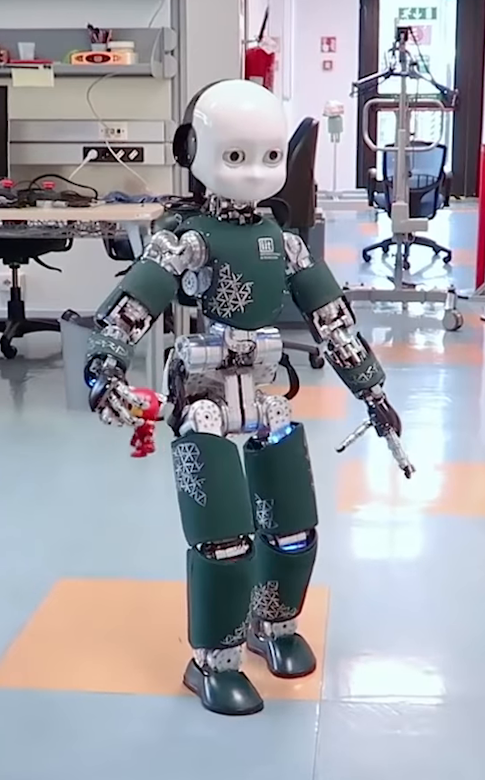
\includegraphics[width=\columnwidth]{chapter_simplified_benchmarking/figures/step1.png}
    \end{subfigure}
    \hfill
           \begin{subfigure}[b]{0.32\textwidth}
        \centering
        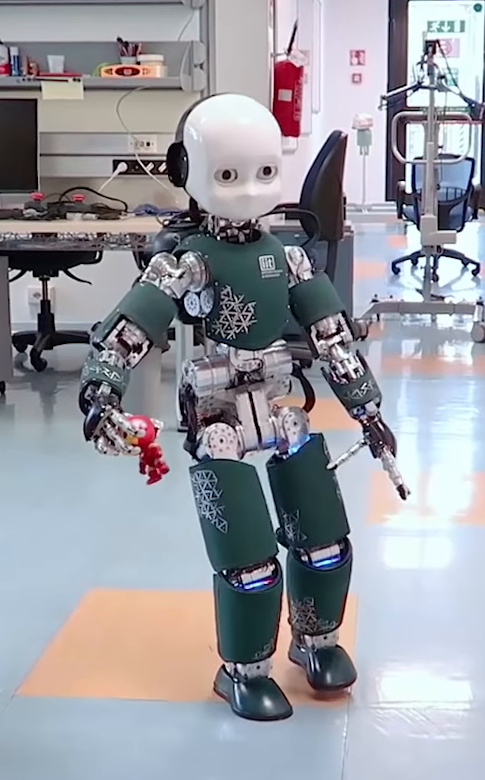
\includegraphics[width=\columnwidth]{chapter_simplified_benchmarking/figures/step2.png}
    \end{subfigure}
    \hfill
           \begin{subfigure}[b]{0.32\textwidth}
        \centering
        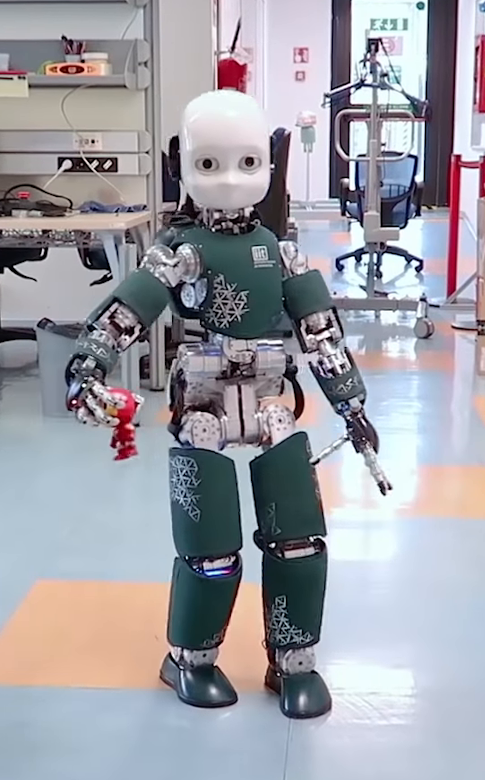
\includegraphics[width=\columnwidth]{chapter_simplified_benchmarking/figures/step3.png}
    \end{subfigure}
    \caption{The iCub robot walks with the 3 layer controller architecture of Figure~\ref{fig:three-layer-simplified-benchmarking}.}
    \label{fig:icub_walking_simplified}
\end{figure}

\section{Results}
\label{sec:results_simplified_benchmarking}
In this section, we present experiments obtained with several implementations of the simplified model controllers, namely: the \emph{instantaneous} and the \emph{predictive} controllers.

To benchmark the different simplified model controllers, we test the algorithms on the iCub humanoid robot v2.7 -- Section~\ref{sec:icub2.7}. We attach the simplified control layer to the three-layer controller architecture shown in Figure~\ref{fig:three-layer}. In this framework, the whole-body control layer implements the kinematics-based whole-body QP presented in section~\ref{sec:ik_qp}. Figure~\ref{fig:icub_walking_simplified} shows the humanoid robot iCub walking with the simplified models controller presented in this chapter.

The control architecture runs on the iCub head's computer, namely a 4-th generation Intel \textsuperscript{\tiny\textregistered} Core i7 @ $\SI{1.7}{\giga \hertz}$. In any of its implementations, the architecture takes (on average) less than $\SI{3}{\milli \second}$ to evaluate its output. The code is open source completely developed in C++: \href{https://github.com/robotology/walking-controllers}{\texttt{https://github.com/robotology/walking-controllers}}. The MPC problem presented in Section~\ref{predictive-control} is solved using the OSQP~\citep{Stellato2018} library~\footnote{Since our code is  written in pure C++, the QP problem is written by means of \texttt{osqp-eigen} a C++ wrapper for OSQP \href{https://github.com/robotology/osqp-eigen}{\texttt{https://github.com/robotology/osqp-eigen}}}.


Table~\ref{tab:max_velocity} summarizes the maximum velocities achieved using the different implementations of the control architecture. In particular, the labels \emph{instantaneous} and \emph{predictive} mean that the associated layer generates its output considering inputs and references either at the single time $t$ or for a time window, respectively. The labels, \emph{velocity} and \emph{position} control, instead, mean that the layer outputs are either desired joint velocities or position, respectively -- see Section~\ref{subsubsec-pos-vel-control}. 

\begin{table}[b]
    \centering
    \caption{Maximum forward straight walking velocities achieved using different implementations of the control architecture.
    }
    \begin{tabular}{cc|c}
         \begin{tabular}{@{}c@{}}Simplified Model  Control\end{tabular} &
         \begin{tabular}{@{}c@{}}Whole-Body QP Control\end{tabular} &
         \begin{tabular}{@{}c@{}}Max Straight Velocity (m/s)\end{tabular}\\
        \hline
        Predictive  & Velocity  &  0.1563\\
        Predictive  & Position  & 0.1645\\
        Instantaneous  & Velocity  &  0.1809\\
        Instantaneous  & Position  & 0.3372
    \end{tabular}
    \label{tab:max_velocity}
\end{table}

Let us remark that all the implemented control architectures exploit the controller presented in Section~\ref{ZMP-CoM-Controller} to attempt the stabilization of the desired center of pressure and desired center of mass position and velocity. The performance of this controller is highly dependent on the gains $K_{zmp}$ and $K_{com}$. In particular, we observed that the gains in achieving good tracking during standing and walking were not the same. For this reason, we implemented a gain-scheduling technique depending on whether the robot is walking or standing. The transition between the two sets of gains is smoothed with a minimum jerk trajectory \citep{Pattacini2010}.


To compare the simplified models controllers, we decided to perform two main experiments. These two experiments represent the maximum robot velocity that has been achieved with all architectures and the maximum velocity achieved with a specific architecture only -- see Table~\ref{tab:max_velocity}. That is, 
\begin{itemize}
    \item[-] \textbf{Experiment 1}: a forward robot speed of $\SI{0.1563}{\meter \per \second}$;
    \item[-] \textbf{Experiment 2}: a forward robot speed of $\SI{0.3372}{\meter \per \second}$.
\end{itemize}

\begin{figure}[t]
    \centering
    \begin{myframe}{Instantaneous + Position Control}
        \centering
    \begin{subfigure}[b]{0.49\textwidth}
        \centering
        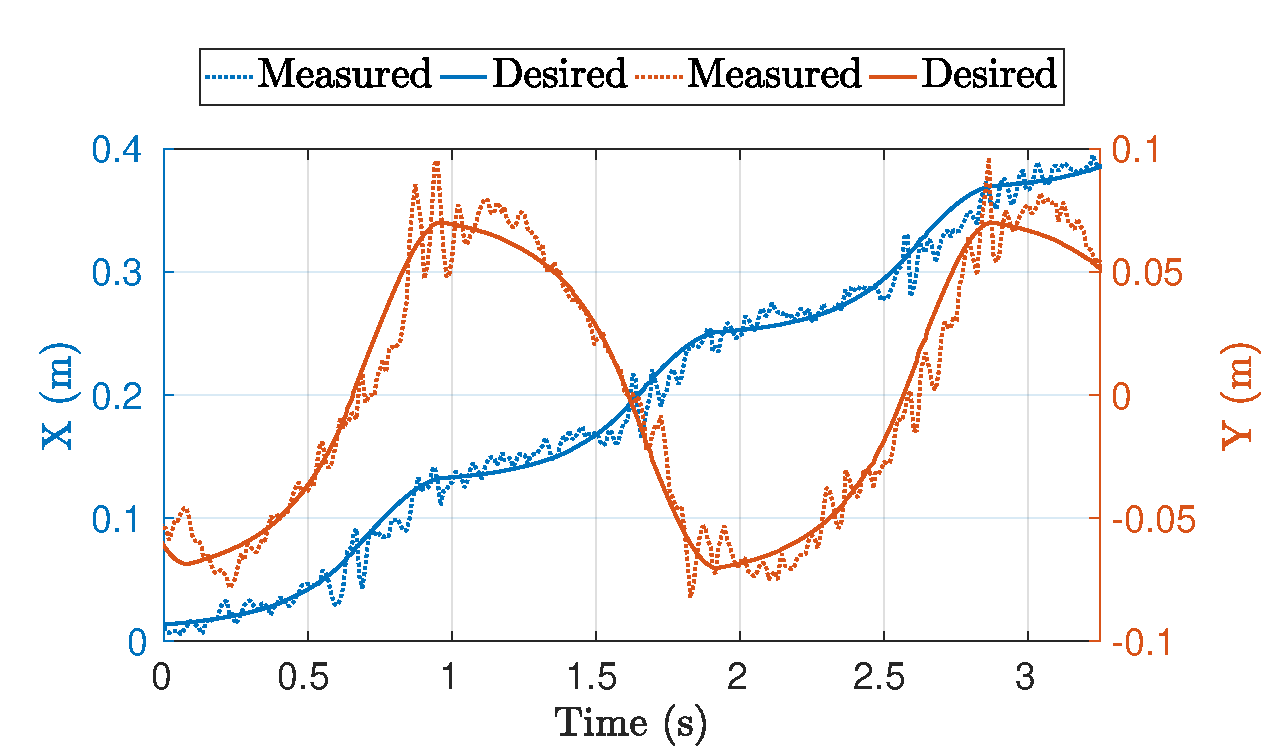
\includegraphics[width=\textwidth]{chapter_simplified_benchmarking/figures/inst_pos-min_vel-dcm.pdf}
        \caption{DCM}
        \label{fig:inst_pos-min_vel-dcm}
    \end{subfigure}
    \hfill
    \begin{subfigure}[b]{0.49\textwidth}
        \centering
        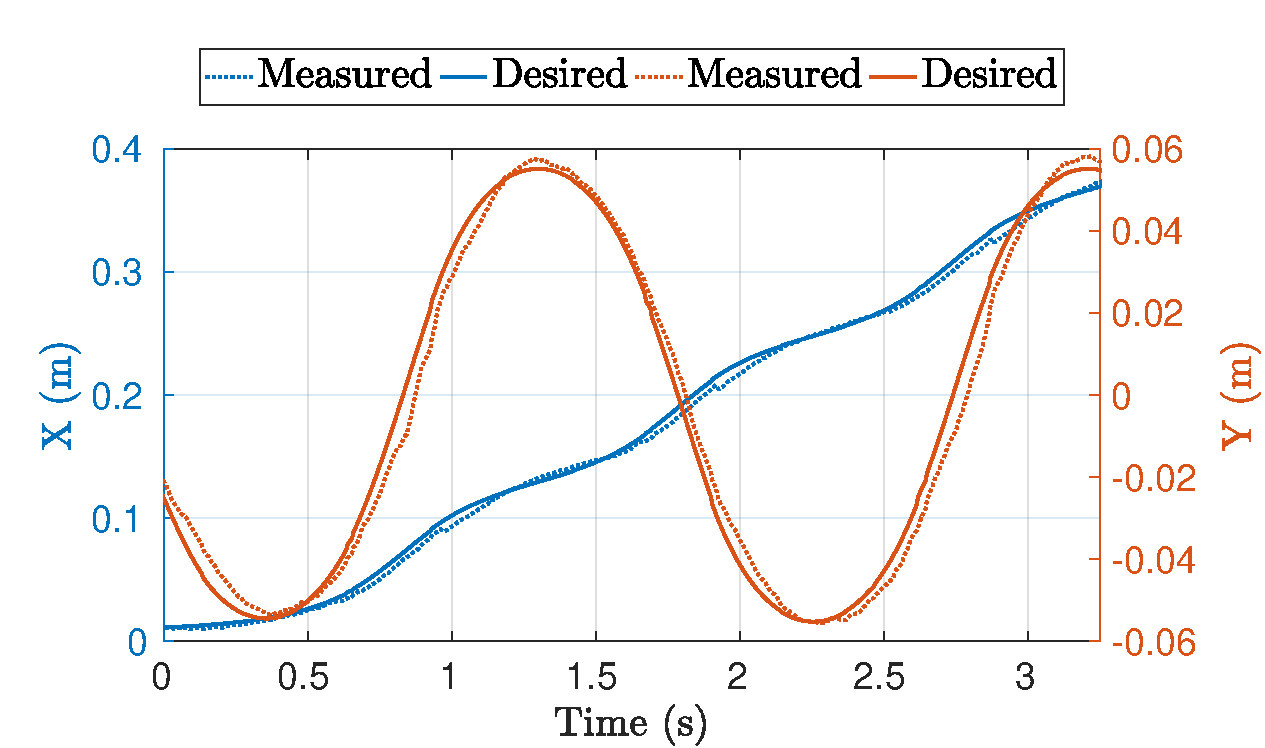
\includegraphics[width=\textwidth]{chapter_simplified_benchmarking/figures/inst_pos-min_vel-com.pdf}
        \caption{CoM}
        \label{fig:inst_pos-min_vel-com}
    \end{subfigure}
    \hfill
    \begin{subfigure}[b]{0.49\textwidth}
        \centering
        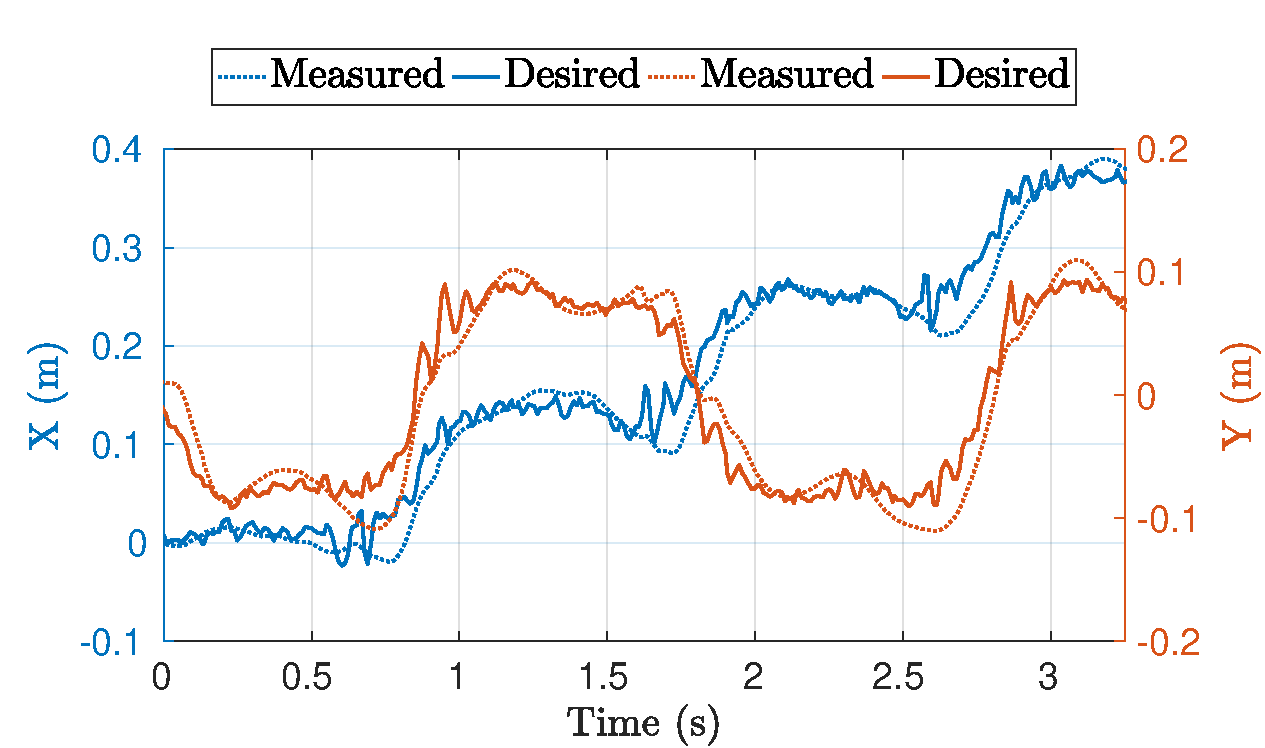
\includegraphics[width=\textwidth]{chapter_simplified_benchmarking/figures/inst_pos-min_vel-zmp.pdf}
        \caption{ZMP}
        \label{fig:inst_pos-min_vel-zmp}
    \end{subfigure}
    \end{myframe}
    \caption{Tracking of the DCM (a), CoM (b) and ZMP (c) using the instantaneous controller with the whole-body controller as position control. Walking velocity:  $\SI{0.19}{\meter \per \second}$.}
\end{figure}

\begin{figure}[t]
    \begin{myframe}{Predictive + Position Control}
     \centering
    \begin{subfigure}[b]{0.49\textwidth}
        \centering
        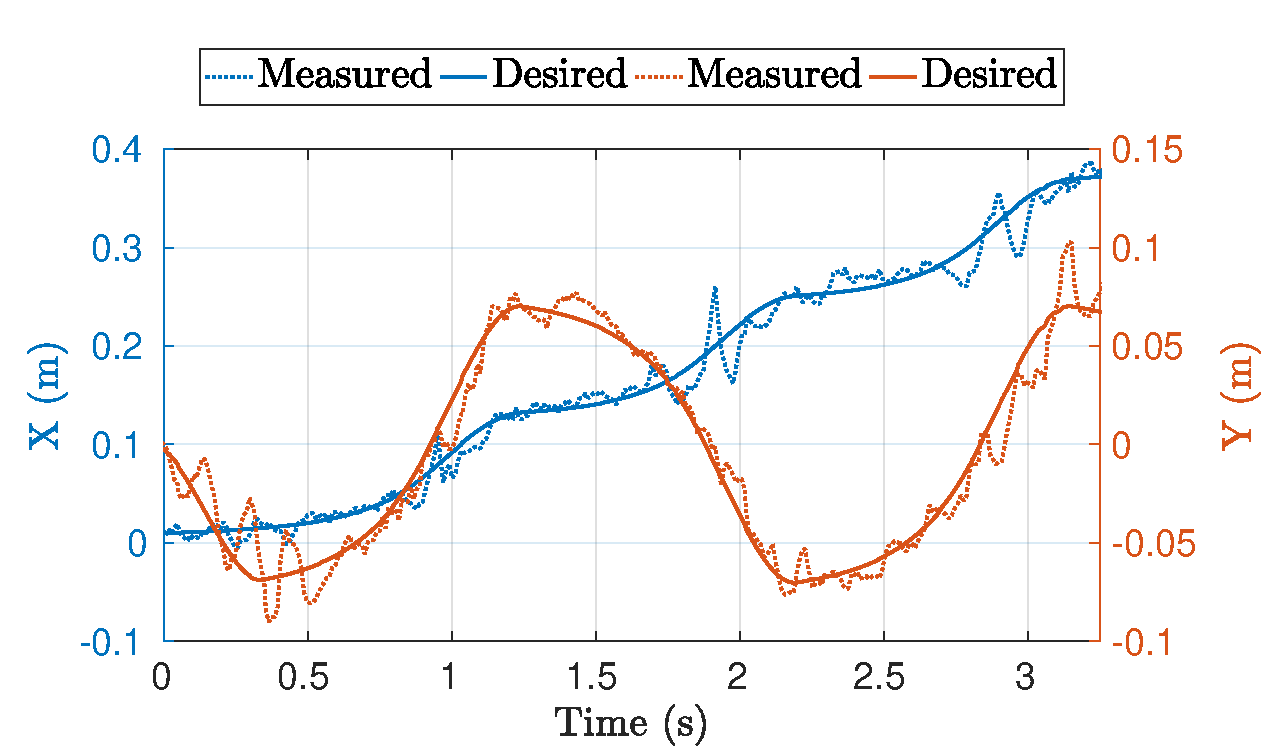
\includegraphics[width=\textwidth]{chapter_simplified_benchmarking/figures/mpc_pos-min_vel-dcm.pdf}
        \caption{DCM}
        \label{fig:mpc_pos-min_vel-dcm}
    \end{subfigure}
    \hfill
    \begin{subfigure}[b]{0.49\textwidth}
        \centering
        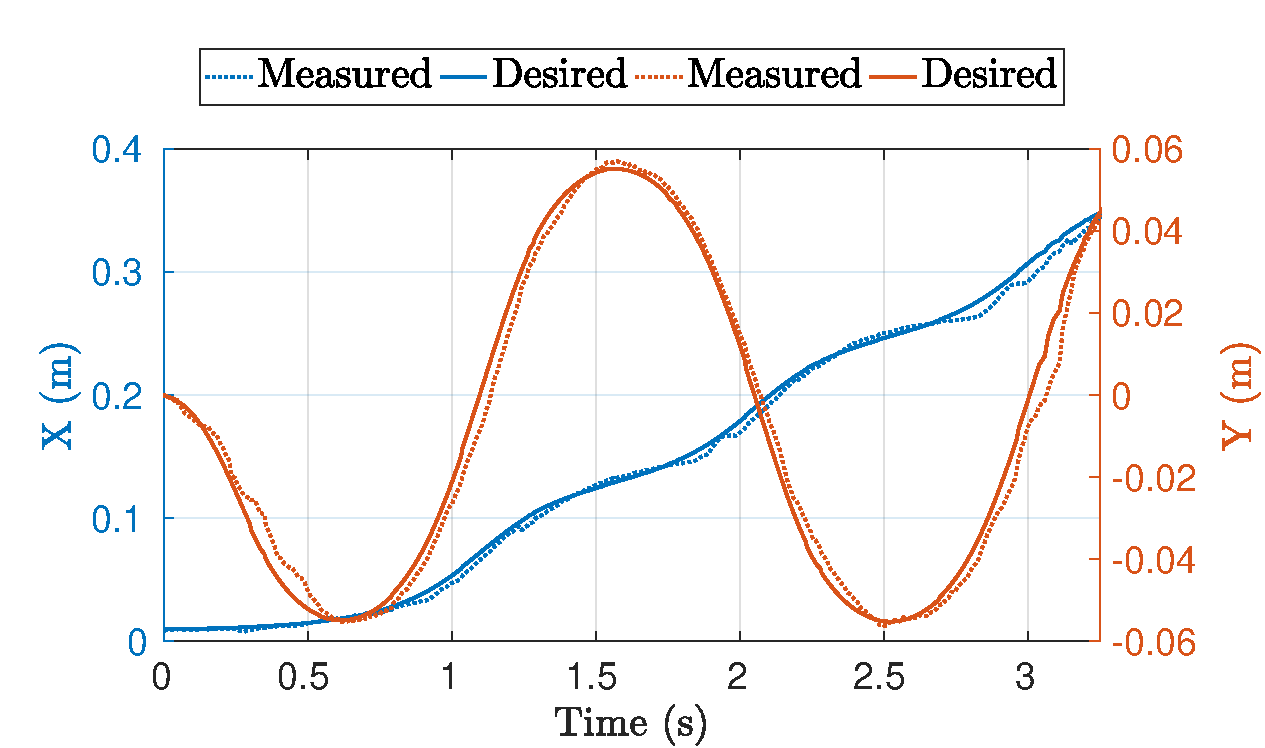
\includegraphics[width=\textwidth]{chapter_simplified_benchmarking/figures/mpc_pos-min_vel-com.pdf}
        \caption{CoM}
        \label{fig:mpc_pos-min_vel-com}
    \end{subfigure}
         \begin{subfigure}[b]{0.49\textwidth}
        \centering
        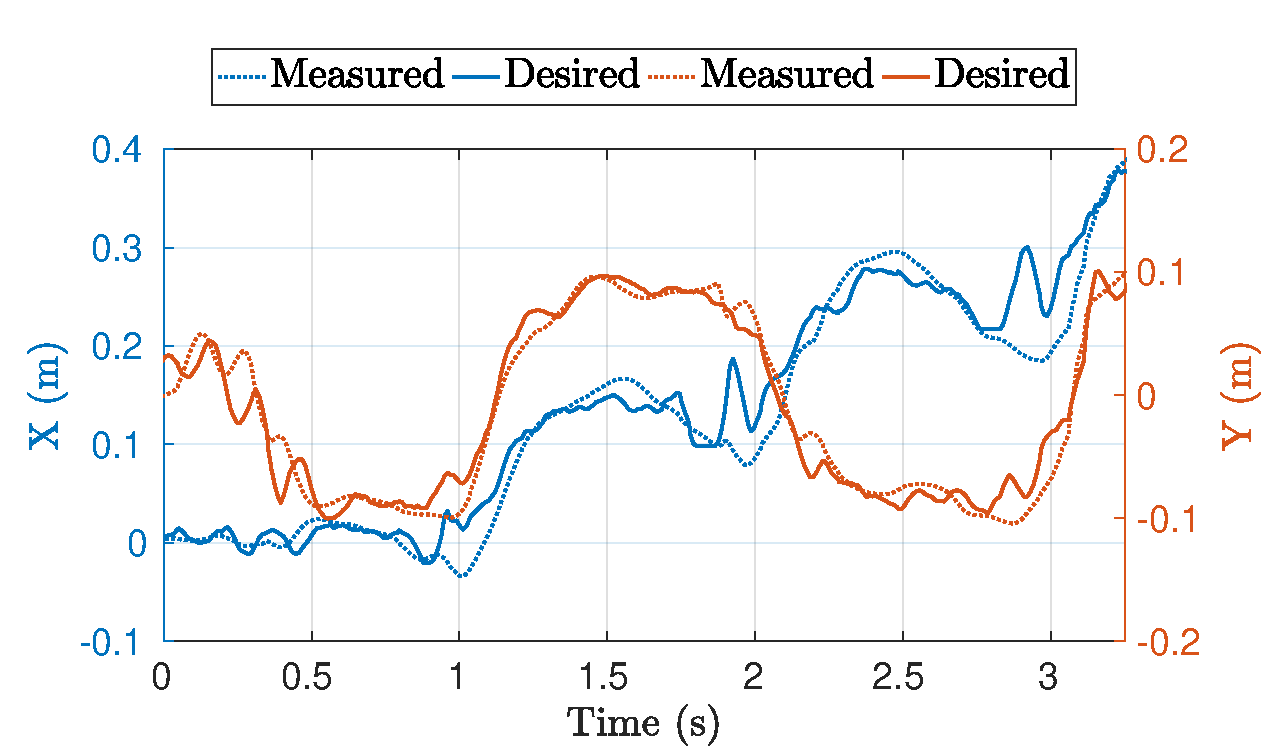
\includegraphics[width=\textwidth]{chapter_simplified_benchmarking/figures/mpc_pos-min_vel-zmp.pdf}
        \caption{ZMP}
        \label{fig:mpc_pos-min_vel-zmp}
    \end{subfigure}
    \end{myframe}
    \caption{Tracking of the  DCM (a), CoM (b) and ZMP (c) using the MPC and the whole-body controller as position control. Walking velocity:  $\SI{0.19}{\meter \per \second}$.}
\end{figure}
\begin{figure}[t]
     \vspace*{-0.1cm}
    \begin{myframe}{Instantaneous + Position Control}
    \centering
        \begin{subfigure}[b]{0.49\textwidth}
        \centering
        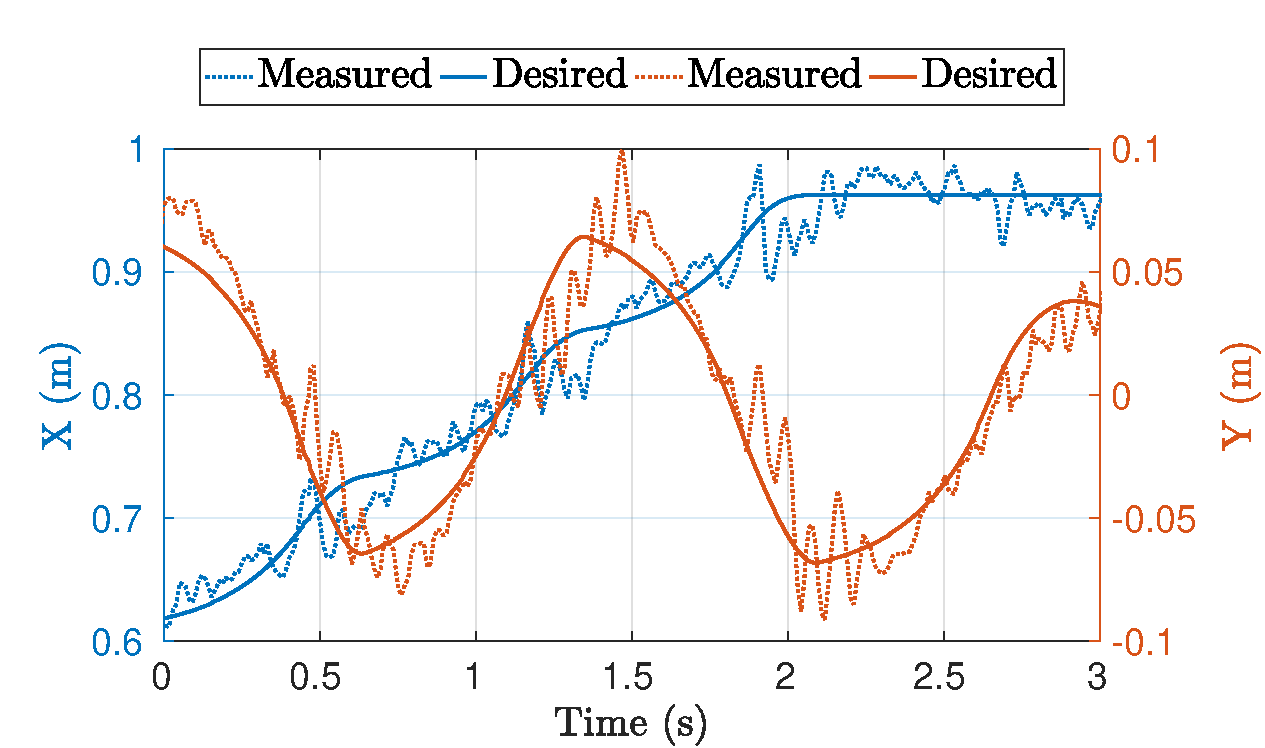
\includegraphics[width=\textwidth]{chapter_simplified_benchmarking/figures/inst_pos-max_vel-dcm.pdf}
        \caption{DCM}
        \label{fig:inst_pos-max_vel-dcm}
    \end{subfigure}
    \hfill
     \begin{subfigure}[b]{0.49\textwidth}
        \centering
        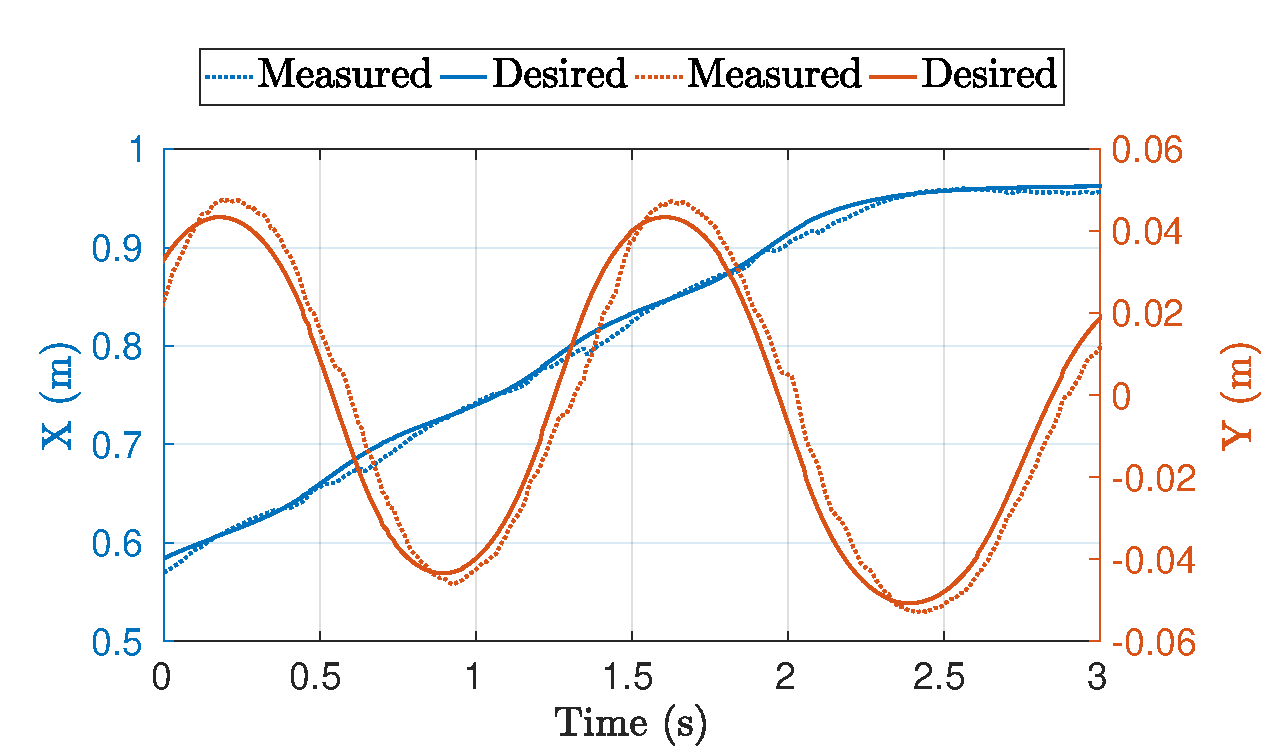
\includegraphics[width=\textwidth]{chapter_simplified_benchmarking/figures/inst_pos-max_vel-com.pdf}
        \caption{CoM}
        \label{fig:inst_pos-max_vel-com}
    \end{subfigure}
    \hfill
    \begin{subfigure}[b]{0.49\textwidth}
        \centering
        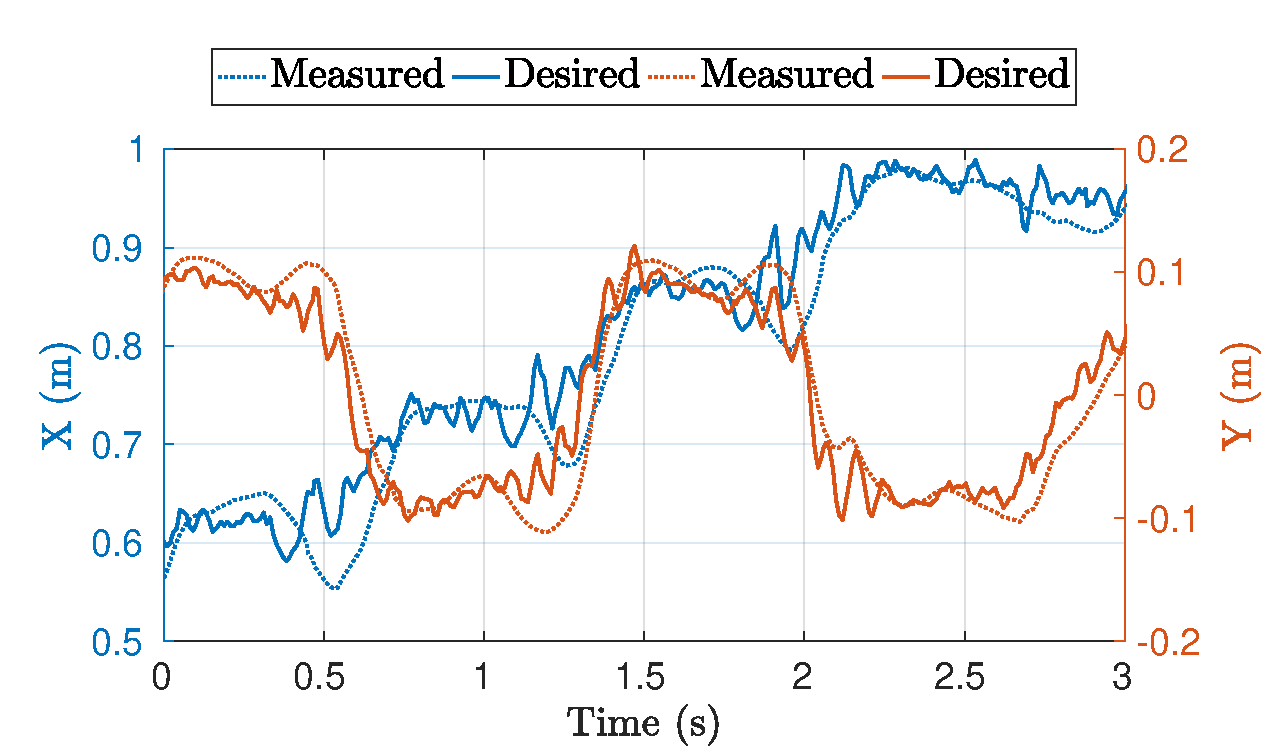
\includegraphics[width=\textwidth]{chapter_simplified_benchmarking/figures/inst_pos-max_vel-zmp.pdf}
        \caption{ZMP}
        \label{fig:inst_pos-max_vel-zmp}
    \end{subfigure}
    \end{myframe}
    \caption{Tracking of the DCM (a), CoM (b) and ZMP (c) with the instantaneous and whole-body QP control as position.  Walking velocity: $\SI{0.41}{\meter \per \second}$.}
\end{figure}
\begin{figure}[t]
    \begin{myframe}{Predictive + Position Control}
    \centering
    \begin{subfigure}[b]{0.49\textwidth}
        \centering
        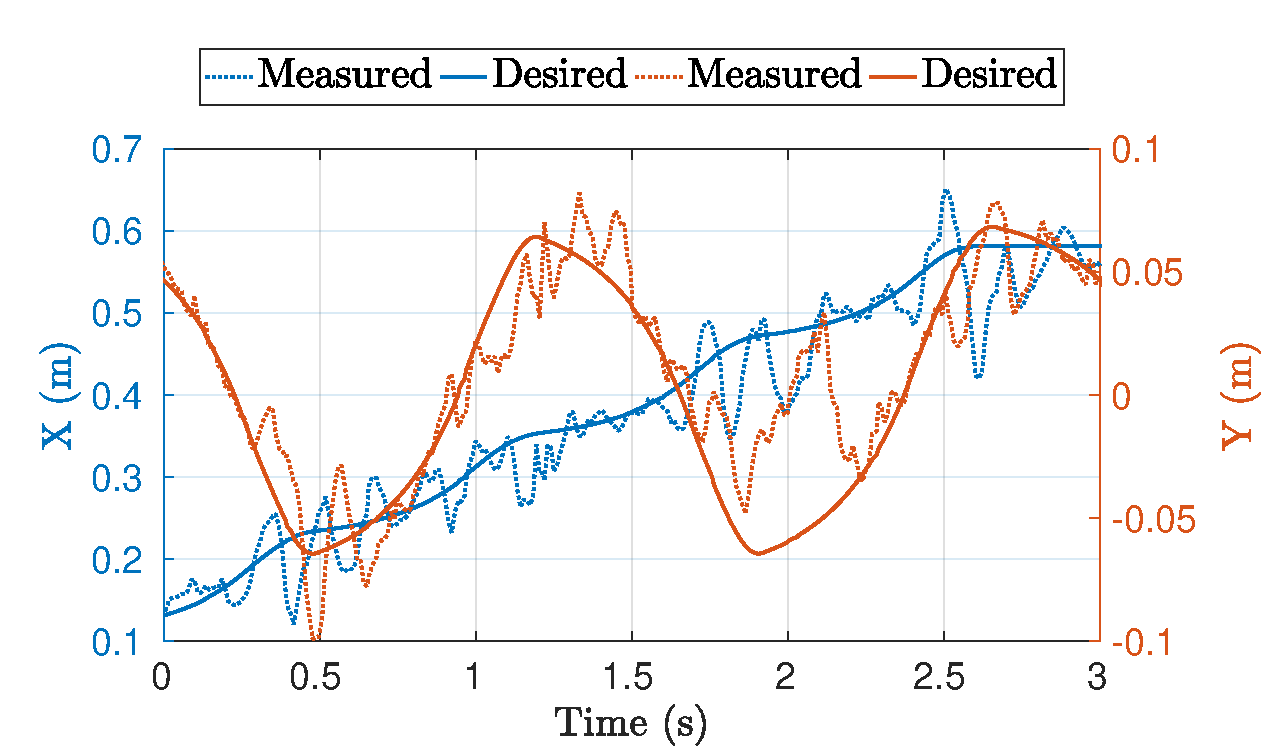
\includegraphics[width=\textwidth]{chapter_simplified_benchmarking/figures/mpc_pos-max_vel-dcm.pdf}
        \caption{DCM}
        \label{fig:mpc_pos-max_vel-dcm}
    \end{subfigure}
    \hfill
     \begin{subfigure}[b]{0.49\textwidth}
        \centering
        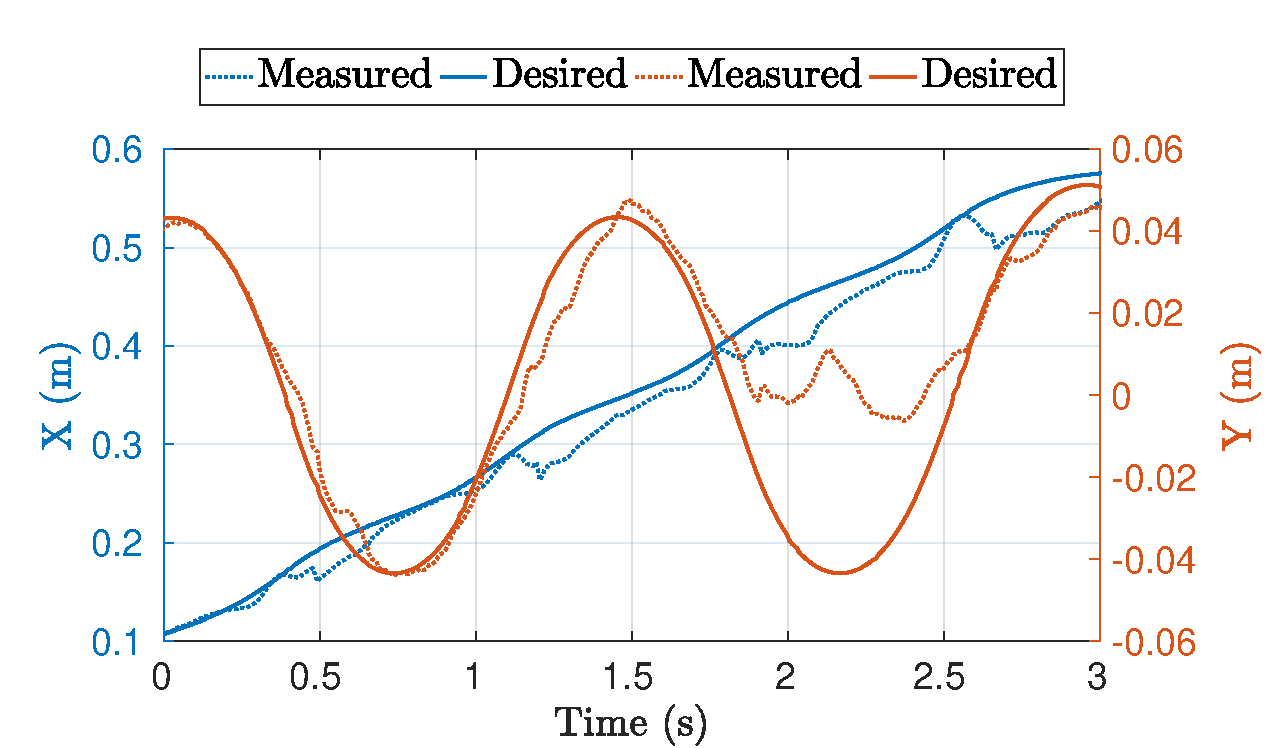
\includegraphics[width=\textwidth]{chapter_simplified_benchmarking/figures/mpc_pos-max_vel-com.pdf}
        \caption{CoM}
        \label{fig:mpc_pos-max_vel-com}
    \end{subfigure}
    \hfill
    \begin{subfigure}[b]{0.49\textwidth}
        \centering
        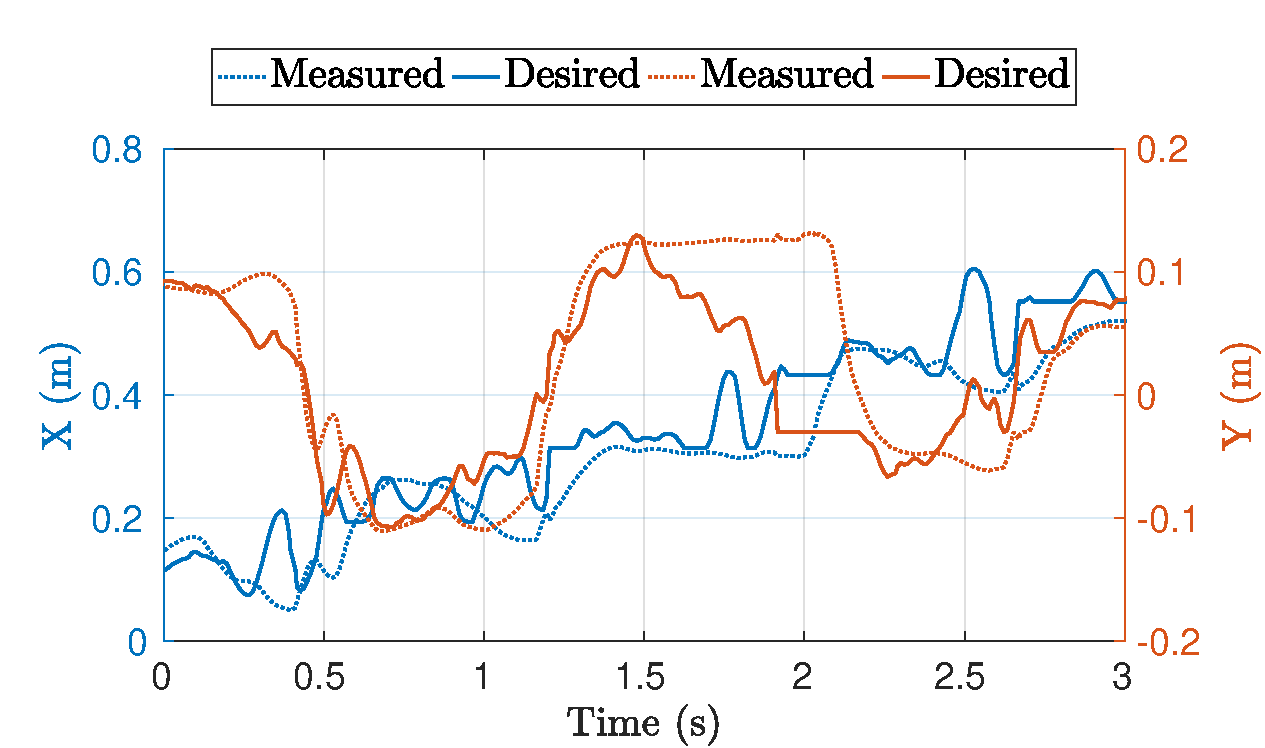
\includegraphics[width=\textwidth]{chapter_simplified_benchmarking/figures/mpc_pos-max_vel-zmp.pdf}
        \caption{ZMP}
        \label{fig:mpc_pos-max_vel-zmp}
    \end{subfigure}
    \end{myframe}
    \caption{Tracking of the  DCM (a), CoM (b) and ZMP (c) with the predictive and whole-body QP control as position control. At $t\approx \SI{2}{\second}$, the robot falls down.  Walking velocity: $\SI{0.41}{\meter \per \second}$.}
    \vskip-0.5cm
\end{figure}

We compare the control laws~\eqref{eq:reactive_dcm} and~\eqref{eq:mpc_solution_simplified}, which both generate a (desired) center of pressure that attempts to stabilize the desired DCM. To simplify the comparison, the controller of the \emph{whole-body QP layer} is kept fixed in this section, and we show and discuss only the results when the robot is position controlled. A complete comparison of the kinematics-based whole-body controllers is presented in Section~\ref{sec:wbc_experimental_results}.
In the following experiments, we set the time horizon of the predictive control to $\SI{2}{\second}$.

\subsection{Experiment 1: a forward robot speed of 0.1563 m s$^{\text{-1}}$}
Figures \ref{fig:inst_pos-min_vel-dcm} and \ref{fig:mpc_pos-min_vel-dcm} show the DCM tracking performances obtained with the instantaneous and predictive controllers, respectively. Both controllers seem to show good tracking performances, and the DCM error is kept below $\SI{5}{\centi \meter}$ in both cases. Note, however, that the instantaneous controller induces faster variations of the measured DCM. This contributes to the overall higher vibrations of the robot. One of the reasons for this variation is that the instantaneous controller~\eqref{eq:reactive_dcm} injects a (desired) center of pressure proportional to the measured DCM, which in turn contains the center of mass velocity. To mitigate this, we may filter the joint velocities appropriately. However, in our case, the joint velocities were not filtered to avoid delays in the measured DCM. Our experience showed that adding a filter to joint velocities is not an easy task, and we did not find the right trade-off for obtaining overall performance improvements. 

Figures~\ref{fig:inst_pos-min_vel-com} and \ref{fig:mpc_pos-min_vel-com} present CoM tracking performances, which are mainly dependent on the ZMP-CoM controller~\eqref{eq:ZMP_controller}. This controller receives the desired DCM values from the \emph{simplified model control} layer, which are obtained with the instantaneous or predictive controllers. In both cases, the CoM error is kept below $\SI{2}{\centi \meter}$. Figures~\ref{fig:inst_pos-min_vel-zmp} and~\ref{fig:mpc_pos-min_vel-zmp} represent the ZMP tracking performance, which is still mainly dependent on the ZMP-CoM controller~\eqref{eq:ZMP_controller}. It is important to note that the desired ZMP is smoother when the \emph{simplified model control} uses the predictive law~\eqref{eq:mpc_solution_simplified} to generate it. Indeed, this is a tunable property that depends on the associated weight in the cost function of the MPC problem. Although this smoother behavior contributes to less robot vibrations, overall robot performance became less reactive and, consequently, less robust to robot falls. Although the extensive hand-made tuning, we were not able to increase the robot velocity when the \emph{simplified model control} used the predictive law~\eqref{eq:mpc_solution_simplified}. 

\subsection{Experiment 2: a forward robot speed of 0.3372 m s$^{\text{-1}}$}
At a robot's desired walking speed of $\SI{0.3372}{\meter \per \second}$, there is initially no significant difference between the DCM tracking obtained with instantaneous and predictive control laws -- see Figures~\ref{fig:mpc_pos-max_vel-dcm} and~\ref{fig:inst_pos-max_vel-dcm} for $t < \SI{1.5}{\second}$. However, fast robot walking velocities require fast variations of the desired CoM and ZMP. This fast variation degrades the performance of the predictive controller around $t = \SI{1.5}{\second}$ -- see Figure~\ref{fig:mpc_pos-max_vel-zmp}. Clearly, these bad performances, in turn, induce poor tracking of the DCM shown in Figure~\ref{fig:mpc_pos-max_vel-dcm} at $t\approx \SI{2}{\second}$, and consequently the robot falls. At this point, one is tempted to increase the gain $K_\text{ZMP}$ of the controller~\eqref{eq:ZMP_controller}, which shall induce a better tracking of the ZMP. Unfortunately, this leads to higher robot oscillations induced by the noise on the estimated ZMP. And, as a consequence, the robot falls. 

We can conclude that the \emph{predictive simplified control} is much less robust than the \emph{instantaneous simplified control} with respect to ZMP tracking errors. Adding a low-pass filter to the ZMP measurement may improve the overall performance. However, in our case, adding filters led to slower system response and, consequently, to the robot falling.



\section{Conclusions \label{sec:conclusions_flexible_joint}}
This chapter presents the design of a whole-body QP control layer for a humanoid robot affected by link flexibility. We model the flexibility by introducing equivalent passive joints that simulate the motion caused by the link deformation.
We then considered the passive joints position and velocity as state of the floating base system dynamics. Thanks to this choice, we develop a whole-body controller that implicitly considers the joint flexibility in the stabilization problem. 
The chapter also details the design of an estimator that aims at computing the flexible joint state in real-time. 
\par
The proposed approach is validated in a simulated version of the TALOS humanoid robot, where its hip flexibility has a significant impact while performing locomotion tasks. Moreover, the architecture is then compared with a whole-body controller that considers all links of the robot rigid.
\par
As a future work, we plan to mitigate the discontinuity of the contact forces by performing a smother transition between contiguous support phases. We also plan to make a detailed comparison with other state-of-the-art controllers that
consider the flexibility of the robot link~\citep{Villa2022TorqueFlexibility}. In addition, we plan to validate the architecture on the real robot.


